\documentclass[a4paper,titlepage]{article}

\title{催化循环的进一步理解之能量跨度模型}
\author{聂万}
\date{2021.04.18}
\usepackage{lmodern}   % fontsize related
\usepackage{amsmath}
\usepackage{ctex}
\usepackage{mathtools}
\usepackage{graphicx}
\usepackage{tikz}
\usepackage{float}

% new commands
\newcommand*\circled[1]{\tikz[baseline=(char.base)]{
    \node[shape=circle, draw, inner sep=1pt,
        minimum height=12pt] (char) {#1};}}
\newcommand{\bigabs}[1]{\Bigl \lvert #1 \Bigr \rvert}

\graphicspath{ {./images/} }
\pagestyle{headings}


\begin{document}

{
\let\clearpage\relax
\maketitle
}

\
\vfil
\hfil
这份材料主要参考了SEBASTIAN KOZUCH和SASON SHAIK的文章。
\footnote{Acc. Chem. Res. 2011, 44, 101–110;
J. Am. Chem. Soc. 2006, 128, 3355–3365}
由于包含了笔者个人的理解,若读者发现错误请不吝赐教。
\footnote{本材料的\LaTeX{}代码已于github开源。\textit{https://github.com/akaruinw/chem}}
\hfil
\vfil

\newpage
\section*{TOF与能量的精确关系式}
\begin{figure}[h]
  \centering
  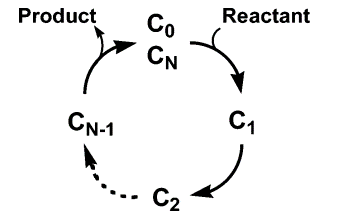
\includegraphics{N_steps}
  \caption{$N$个步骤的催化循环}
  \label{fig:N stepts}  % label should after caption
\end{figure}

对于一个有$N$个步骤的催化循环来说(图\ref{fig:N stepts}),
根据稳态近似理论可知,
整个反应的$r$等于每个分步的反应速率$r_i$。
\begin{equation}\label{eq:substeps}
    r = k_1C_0 - k_{-1}C_{1} =k_2C_1 - k_{-2}C_{2}=...=k_NC_{N-1} - k_{-N}C_{N}
\end{equation}
以一个有四步的催化反应为例。$(\ref{eq:substeps})$可以继续改写为:
\begin{equation*}
\begin{pmatrix}
   k_1 & -k_{-1} & 0 & 0  \\
   0 & k_2 & -k_{-2} & 0  \\
   0 & 0 & k_3 & -k_{-3}  \\
  -k_{4} & 0 & 0 & k_4  \\
\end{pmatrix}
\begin{pmatrix}
  C_{0}  \\
  C_{1}  \\
  C_{2}  \\
  C_{3}
\end{pmatrix}
=
\begin{pmatrix}
  r  \\
  r  \\
  r  \\
  r
\end{pmatrix}
\end{equation*}
Christiansen\footnote{J. A. AdV. Catal. 1953, 5, 311.}
利用$(\ref{eq:substeps})$的矩阵形式继续推导得到了:
\begin{equation}\label{eq:TOF=Delta/M}
  TOF = \frac{\Delta{}}{M}
\end{equation}
其中$\Delta{}$是各步骤正负反应速率常数的积的差:
\begin{equation}
  \Delta{}=k_1k_2\hdots{}k_N-k_{-1}k_{-2}\hdots{}k_{-N}
\end{equation}
$M$是$\hat{M}$矩阵各元素的和:

\begin{equation}
  \hat{M}=
  \begin{psmallmatrix}
     k_{2}k_{3}k_{4}\hdots{}k_{N} & k_{-1}k_{3}k_{4}\hdots{}k_{N} & k_{-1}k_{-2}k_{4}\hdots{}k_{N} &\hdots{}& k_{-1}k_{-2}k_{-3}\hdots{}k_{-(N-1)}\\
     k_{3}k_{4}\hdots{}k_{N}k_{1} & k_{-2}k_{4}\hdots{}k_{N}k_{1} & k_{-2}k_{-3}\hdots{}k_{N}k_{1} &\hdots{}& k_{-2}k_{-3}\hdots{}k_{-(N-1)}k_{-N}\\
     \vdots{} & \vdots{} & \vdots{} & \ddots & \vdots \\
     k_{N}k_{1}k_{2}\hdots{}k_{N-2} & k_{-(N-1)}k_{1}k_{2}\hdots{}k_{N-2} & k_{-(N-1)}k_{-N}k_2\hdots{}k_{N-2} & \hdots{}&k_{-N}k_{-(N-1)}k_{-1}\hdots{}k_{-(N-3)}\\
     k_{1}k_{2}k_{3}\hdots{}k_{N-1} & k_{-N}k_{2}k_{3}\hdots{}k_{N-1} & k_{-N}k_{-1}k_{3}\hdots{}k_{(N-1)} &\hdots{}& k_{-N}k_{-1}k_{-2}\hdots{}k_{-(N-2)}\\
  \end{psmallmatrix}
\end{equation}


为了将$(\ref{eq:TOF=Delta/M})$中的反应速率常数转换为能量,我们需要借助Erying Equation:
\begin{equation}\label{eq:Erying}
\begin{split}
k_i = \frac{k_BT}{h}e^{-\Delta G_i^{\neq}/RT} = \frac{k_BT}{h}e^{(I_{i-1} - T_i)/RT}
\\
k_{-i} = \frac{k_BT}{h}e^{-\Delta G_{-i}^{\neq}/RT} = \frac{k_BT}{h}e^{(I_{i} - T_i)/RT}
\end{split}
\end{equation}
这其中$I_i$指的是第$i$个中间体的自由能,类似的$T_i$指的是第$i$个过渡态的自由能。这里$k_{-i}$的下标$-i$指的是负反应。
结合$(\ref{eq:TOF=Delta/M})$与$(\ref{eq:Erying})$可以得到:
\begin{equation}\label{eq:TOFcomplete}
\begin{split}
  TOF
  & =
  \frac{k_BT}{h}
  \frac{e^{-\Delta{G}_{r}/RT}-1}{\sum\limits_{i,j=1}^{N}e^{(T_i-I_j-\delta{}G_{i,j}^{'})/RT}}
  = \frac{\Delta{}}{M}
  \\
  \delta{}G_{i,j}^{'} & =
                  \begin{cases}
                  \Delta{G}_r & \text{if $i > j$}\\
                  0 & \text{if $i \leq j$}
                 \end{cases}
\end{split}
\end{equation}

为了理解$(\ref{eq:TOFcomplete})$我们可以将其类比为欧姆定律。如果TOF是电流的话,
$\Delta{}$就是电势差,$M$为电阻。
TOF与反应能$\Delta{G}_r$成反比,$\Delta{G}_r$越负,TOF越大,当$\Delta{G}_r=0$时TOF为0。
“电阻”来自于所有中间体和过渡态组合能量差的指数和。
当过渡态在中间体后面时($i>j$),能量差还要再减去反应能。

\begin{figure}[h]
  \centering
  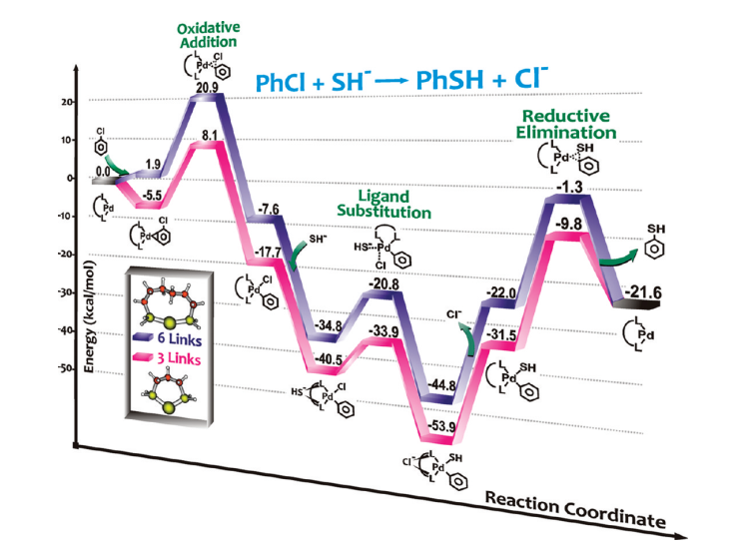
\includegraphics[width=12cm, height=6cm]{fig2}
  \caption{Pd催化的偶联反应}
  \label{fig:energies}
\end{figure}
利用$(\ref{eq:TOFcomplete})$可以分别求出图\ref{fig:energies}中$n=3$和$n=6$时的TOF,
并且$TOF(n=3)/TOF(n=6) = 1.45$

\section*{能量跨度模型以及TDI/TDTS的确立}
\subsection*{TOF与能量的近似关系式}
基于两个假设:
$\begin{cases}
  \text{分子中的$-1$项可以被忽略}\\
  \text{分母只由一组能量跨度较大的$T_i$和$I_j$决定}
\end{cases}$,
\textit{放热反应}的公式$(\ref{eq:TOFcomplete})$可以被进一步简化为:
\begin{equation}\label{eq:TOFappro}
  TOF = \frac{k_BT}{h}e^{-\delta{E}/RT}
\end{equation}
其中:
\begin{equation}\label{eq:tdts}
  \begin{split}
    \delta{E}=
      \begin{cases}
        T_{TDTS}-I_{TDI}   & \text{TDTS在TDI后出现}\\
        T_{TDTS}-I_{TDI}+\Delta{G}_r  & \text{TDTS在TDI前出现}\\
      \end{cases}
  \end{split}
\end{equation}
具体的推导如下:
\begin{equation}
\begin{split}
  TOF(i>j)
  & = \frac{k_BT}{h}\frac{e^{-\Delta{G}_r/RT}}{e^{(T_i-I_j-\Delta{G}_r)/RT}}\\
  & = \frac{k_BT}{h}\frac{1}{e^{(T_i-I_j)/RT}}\\
  & = \frac{k_BT}{h}e^{-\delta{E}/RT}\\
  TOF(i\leq{}j) & = \frac{k_BT}{h}\frac{e^{-\Delta{G}_r/RT}}{e^{(T_i-I_j)/RT}}\\
  & = \frac{k_BT}{h}\frac{1}{e^{(T_i-I_j+\Delta{G}_r)/RT}}\\
  & = \frac{k_BT}{h}e^{-\delta{E}/RT}
\end{split}
\end{equation}

公式\ref{eq:tdts}中的\textbf{TDTS}全称为TOF-determining trainsition state,
\textbf{TDI}全称为TOF-determining intermediate。
在一些文献中TDI又被称为resting state,TDTS被称为rate-limiting TS。
这两个物质的组合代表了最大的能量跨度,很大程度上决定了反应的速率,
因此我们可以将$\delta{E}$称为
“\textit{整个催化循环的表观活化能(apparent activation energy of the cycle)}”。

现在我们在利用近似公式(\ref{eq:TOFappro})和(\ref{eq:tdts})
来计算一下图\ref{fig:energies}中两条反应路线的TOF。
$n=3$时,TDI为-53.9 kcal/mol的中间体,TDTS是还原消除的过渡态(9.8 kcal/mol),
利用公式可得$TOF=1.2\times{}10^{-16}h^{-1}$。
$n=6$时,TDI为-44.8 kcal/mol的中间体,TDTS为氧化加成的过渡态(20.9 kcal/mol),
由公式可得$TOF=1.2\times{}10^{-16}h^{-1}$。$TOF(n=3)/TOF(n=6) = 1$,
接近用精确公式求得的比例(1.45)。这里可能存在为什么$n=6$时,TDTS是氧化加成过渡态的疑问,
这个我们在下面解释一下。

\subsection*{TDI/TDTS如何判断}
\textit{对于一个放热反应来说TDI和TDTS是能够将能量跨度$\delta{E}$最大化的一个组合。}
此处的\textit{“能量跨度”}并不是单纯的过渡态和中间体的能量差,还要考虑反应能,
具体原因参见公式(\ref{eq:tdts})中的$\delta{E}$。
TDI一般情况下是整个催化循环中能量比较低的中间体(注意不一定是最低),
但是TDTS有可能在TDI之前出现,也有可能再其之后出现。

我们以图\ref{fig:energies}为例,在这两种情况中,TDTS可能是氧化加成或还原消除的过渡态。
$n=3$时,TDTS可能是8.1(kcal/mol)的过渡态,也有可能是-9.8的过渡态。
根据公式(\ref{eq:tdts}),两种情况的能量跨度分别为:
\begin{center}
$\delta{E}=
\begin{cases}
    T - I + \Delta{G_r} & = 8.1 - (-53.9) + (-21.6) = 40.4\\
    T - I  & = -9.8 - (-53.9) = 44.1\\
\end{cases}$
\end{center}
44.1大于40.4,因此可以判断$n=3$时,还原消除的过渡态是TDTS。

$n=6$时,TDTS可能是20.9的过渡态,也有可能是-1.3的过渡态,两种情况的能量跨度分别为:
\begin{center}
$\delta{E}=
\begin{cases}
    T - I + \Delta{G_r} & = 20.9 - (-44.8) + (-21.6) = 44.1\\
    T - I &  = -1.3 - (-44.8) = 43.5\\
\end{cases}$
\end{center}
44.1大于43.5,因此$n=6$时,氧化加成的过渡态是TDTS。

通过以上两种情况的分析,我们可以发现
\circled{1}\textit{整个反应的速率是受到两个states影响的,而不是单独的一步反应。}
\circled{2}\textit{TDTS既不一定是能量最高的过渡态,也不一定是活化能最高的过渡态}。

TDI/TDTS的应用可以参见Carvajal
\footnote{Organometallics 2009, 28, 3656–3665.}等人的文章。
应用简化配体计算整个催化循环路线后可以找到反应的TDI/TSTS,
计算真实配体的TDI/TDTS后即可得到真实的TOF(图\ref{fig:tdi/tdts_utility})。

\begin{figure}[H]
  \centering
  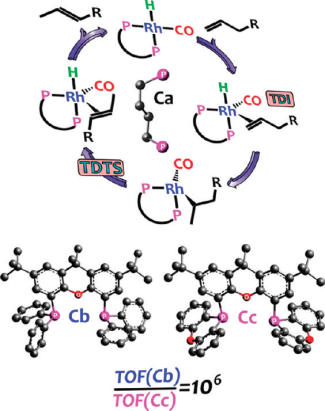
\includegraphics[scale=0.5]{fig3}
  \caption{Rh催化的烯烃异构化反应。催化循环用\textbf{Ca}配体计算,找到TDI/TDTS后
  分别计算\textbf{Cb}和\textbf{Cc}的TDI/TDTS。}
  \label{fig:tdi/tdts_utility}
\end{figure}

\section*{TOF控制度(degree of TOF control)}
根据Campbell\footnote{Top. Catal. 1994, 1, 353–366;  J. Catal. 2001, 204, 520–524}
对\textit{速率控制度(degree of rate control)}的定义,
Kozuch定义了\textit{TOF控制度(degree of rate control)}:
\begin{equation}\label{eq:TOF_control_def}
  X_{TOF,E_i} =
  \bigabs
  {
  \frac{1}{TOF}\frac{\partial{TOF}}{\partial{E_i}}
  } =
  \bigabs
  {
  \frac{\partial{\ln{TOF}}}{\partial{E_i}}
  }
\end{equation}
其中$E_i$可以是过渡态的能量,也可以是中间体的能量。
这一概念的提出是为了定量描述反应历程中各个物质对TOF的影响。
由于$X_{TOF,Ei}$与TOF对$E_i$的偏导数的绝对值成正比,
因此$X_{TOF,Ei}$的值越大,表明$E_i$对TOF的影响越大,也越有可能是TDI/TDTS。

接下来让我们分别求出过渡态和中间体的$X_{TOF,E_i}$来看一下长什么样子。
根据公式$(\ref{eq:TOFcomplete})$,$E_i$为过渡态能量$T_i$时:
\begin{equation}\label{eq:TOF/Ti_partial}
  \frac{\partial{TOF}}{\partial{T_i}} =
    -\frac{k_BT}{h}
    (e^{-\Delta{G}_r/RT}-1)
    (\sum\limits_{ij}e^{(T_i-I_j-\delta{G}_{i,j}^{'})/RT})^{-2}
    (\sum\limits_{j}e^{(T_i-I_j-\delta{G}_{i,j}^{'})/RT})
    \frac{1}{RT}
\end{equation}
结合$(\ref{eq:TOF_control_def})$和$(\ref{eq:TOF/Ti_partial})$,我们可以得到:
\begin{equation}\label{eq:TOF_Ti_withRT}
\begin{split}
X_{TOF,T_i}
  &= \bigabs{
      \frac{1}{TOF}\frac{\partial{TOF}}{\partial{T_i}}
      } \\
  &= (\sum\limits_{ij}e^{(T_i-I_j-\delta{G}_{i,j}^{'})/RT})^{-1}
      (\sum\limits_{j}e^{(T_i-I_j-\delta{G}_{i,j}^{'})/RT})
      \frac{1}{RT} \\
  &= \frac
{\sum\limits_{j}e^{(T_i-I_j-\delta{G}_{i,j}^{'})/RT}}
{RT\sum\limits_{ij}e^{(T_i-I_j-\delta{G}_{i,j}^{'})/RT}}
\end{split}
\end{equation}

$E_i$为中间体能量$I_j$时:
\begin{equation}\label{eq:TOF/Ij_partial}
  \frac{\partial{TOF}}{\partial{I_j}} =
    -\frac{k_BT}{h}
    (e^{-\Delta{G}_r/RT}-1)
    (\sum\limits_{ij}e^{(T_i-I_j-\delta{G}_{i,j}^{'})/RT})^{-2}
    (\sum\limits_{i}e^{(T_i-I_j-\delta{G}_{i,j}^{'})/RT})
    \frac{-1}{RT}
\end{equation}
结合$(\ref{eq:TOF_control_def})$和$(\ref{eq:TOF/Ij_partial})$,我们可以得到:
\begin{equation}\label{eq:TOF_Ij_withRT}
\begin{split}
X_{TOF,I_j}
  &= \bigabs{
      \frac{1}{TOF}\frac{\partial{TOF}}{\partial{I_j}}
      } \\
  &= (\sum\limits_{ij}e^{(T_i-I_j-\delta{G}_{i,j}^{'})/RT})^{-1}
      (\sum\limits_{i}e^{(T_i-I_j-\delta{G}_{i,j}^{'})/RT})
      \frac{1}{RT} \\
  &= \frac
{\sum\limits_{i}e^{(T_i-I_j-\delta{G}_{i,j}^{'})/RT}}
{RT\sum\limits_{ij}e^{(T_i-I_j-\delta{G}_{i,j}^{'})/RT}}
\end{split}
\end{equation}

如果我们定义
$
  X_{TOF,E_i} =
  \bigabs{
  \frac{RT}{TOF}\frac{\partial{TOF}}{\partial{E_i}}
  }
$,
$(\ref{eq:TOF_Ti_withRT})$和$\ref{eq:TOF_Ij_withRT}$可以变为:
\footnote{实际上Kozuch定义的TOF没有$RT$项,笔者认为原文这里是个bug}
\begin{equation}\label{eq:TOF_noRT}
  \begin{split}
    X_{TOF,T_i}
    &= \frac
      {\sum\limits_{j}e^{(T_i-I_j-\delta{G}_{i,j}^{'})/RT}}
      {\sum\limits_{ij}e^{(T_i-I_j-\delta{G}_{i,j}^{'})/RT}} \\
    X_{TOF,I_j}
    &= \frac
      {\sum\limits_{i}e^{(T_i-I_j-\delta{G}_{i,j}^{'})/RT}}
      {\sum\limits_{ij}e^{(T_i-I_j-\delta{G}_{i,j}^{'})/RT}}
  \end{split}
\end{equation}
分析公式$(\ref{eq:TOF_noRT})$可以看出,$X_{TOF,E_i}\in (0, 1)$,
其越接近于1,$E_i$对TOF的影响就越大,
并且$\sum{}X_{TOF,T}=1$,$\sum{}X_{TOF,I}=1$。
$X_{TOF}$最大的中间体和过渡态分别对应了TDI/TDTS。
在图\ref{fig:energies}中,$n=3$时只有一个过渡态有较大的$X_{TOF}$。
而$n=6$时,有两个过渡态有较大的$X_{TOF}$,
分别为氧化加成过渡态($X_{TOF}=0.7$)和还原消除过渡态($X_{TOF}=0.3$)。
这解释了为什么用精确公式($\ref{eq:TOFcomplete}$)计算得到的TOF要比
用近似公式($\ref{eq:TOFappro}$)得到的TOF小$30\%$。

\section*{反应物和产物浓度对TOF的影响}
我们在上面讨论的所有内容都是基于了TOF的精确表达式(\ref{eq:TOFcomplete}),
该表达式是由中间体的关系推导得出的,而没有考虑反应物和产物浓度的影响。
虽然一般人们很少讨论反应物和产物浓度对TOF的影响,
但是浓度的影响是确实存在的。对TOF近似表达式的一个扩展如下:
\footnote{详细的推导参见:
J. Phys. Chem. A 2008, 112,
6032–6041; J. Comput. Chem. 32, 978-985}
\begin{equation}\label{eq:TOF_withConcentration}
  TOF = \frac{k_BT}{h}e^{-\delta{E}/RT}\prod{}\frac{[R]}{[P]}
        \Biggr\rvert{}_{\textit{from TDI to TDTS}}
\end{equation}
公式($\ref{eq:TOFappro}$)乘上TDI和TDTS之间所有反应物浓度积与产物浓度积的商。
当反应物浓度增加时或者产物浓度降低时,TOF会相应增加。
TOF与反应物和产物的浓度成线性关系,与中间体和过渡态的能量成指数关系。

\section*{镍催化的偶联反应:能量跨度模型应用举例}
一个有代表性的应用是镍催化的酸酐与有机锌试剂的偶联反应
(图\ref{fig:Ni-bipy_anhydride_Zn})。
Johnson等人
\footnote{J. Am. Chem. Soc. 2007, 129, 2718–2725}
报道了这个反应,作者发现此反应的动力学现象很不寻常:
酸酐的浓度对反应速率没有影响,
TOF与Et\textsubscript{2}Zn的浓度成线性相关直到超过特定浓度后TOF不再增长。
Johnson等人对此现象进行了总结:
\begin{enumerate}
  \item 氧化加成步不是绝速步,因为酸酐的浓度对TOF没有影响。
  \item Et\textsubscript{2}Zn浓度较低时,转金属化步是绝速步,
        因为TOF与Et\textsubscript{2}Zn浓度线性相关。
  \item Et\textsubscript{2}Zn浓度较高时,TOF恒定不变,因此还原消除为绝速步。
\end{enumerate}
\begin{figure}[H]  % the uppercase "H" forces latex to put the figure "HERE"
  \centering
  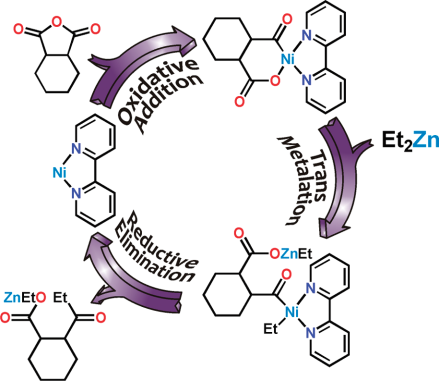
\includegraphics[scale=0.5]{fig4}
  \caption{Ni-bipy催化的酸酐与有机锌试剂的偶联反应。}
  \label{fig:Ni-bipy_anhydride_Zn}  % label should after caption
\end{figure}

随后Kozuch等人
\footnote{\label{paper:TOF_withConcentration}Organometallics 2009, 28, 1303–1308}
对这个反应进行了计算并得到了能量曲线(图\ref{fig:Ni_profile})。
\begin{enumerate}
  \item COD对Ni的配体可以降低氧化加成过渡态的能垒(\textbf{TS\textsubscript{OA}}),
  \item 催化剂为了回到初始状态,最后\textbf{4}会与COD发生配体交换(\textbf{TS\textsubscript{LS}})。
  \item 计算方法高估了熵效应,真实的自由能曲线可能在E+ZPE和G曲线之间。
  \item 在G曲线中,TDI是Ni\textsuperscript{II}化合物\textbf{2},
        而在E+ZPE曲线中TDI是\textbf{2}与Et\textsubscript{2}Zn的络合物\textbf{2Zn}。
  \item 在E+ZPE曲线和G曲线中,TDTS都是\textbf{TS\textsubscript{LS}}。
\end{enumerate}
\begin{figure}[H]  % 'ht' means 'h' or 't'
  \centering
  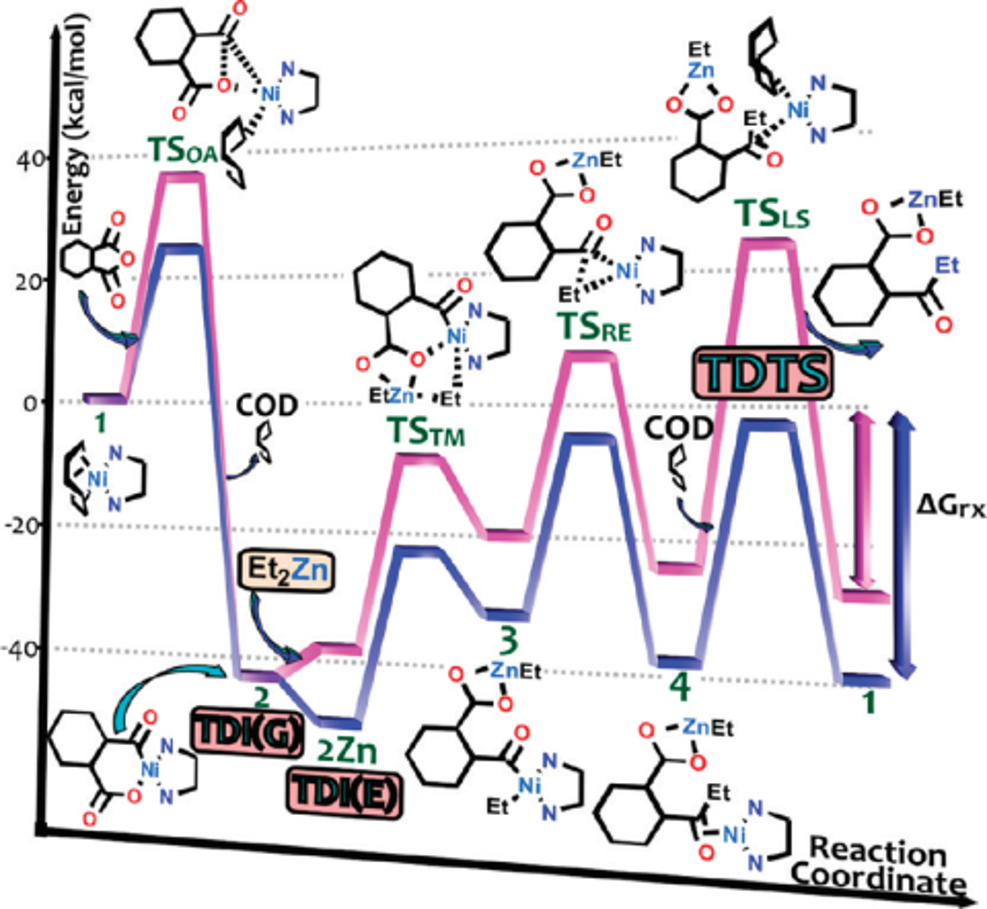
\includegraphics[scale=0.5]{Ni_profile}
  \caption{Ni-bipy催化的酸酐与有机锌试剂的偶联反应能量曲线。
          蓝色曲线表示能量(E+ZPE),粉色曲线表示自由能(G)。}
  \label{fig:Ni_profile}  % label should after caption
\end{figure}

\begin{subequations}  % subequations本身不是math mode,必须在里面指定math mode
  在E+ZPE曲线中,\textbf{2Zn}和\textbf{TS\textsubscript{LS}}之间没有得到产物,
  也没有反应物的参与(不考虑COD,因为其是催化剂的一部分)。
  因此,根据公式\ref{eq:TOF_withConcentration},我们可以得到:
  \begin{equation}\label{eq:Ni_TOF_E}
    TOF(\text{E}) = \frac{k_BT}{h}
                      e^{-[E(\textbf{TS\textsubscript{LS}}) - E(\textbf{2Zn})]}
  \end{equation}
  在G曲线中,\textbf{2}和\textbf{TS\textsubscript{LS}}之间没有得到产物,
  但进入了反应物Et\textsubscript{2}Zn。
  因此,根据公式$(\ref{eq:TOF_withConcentration})$,我们可以得到:
  \begin{equation}\label{eq:Ni_TOF_G}
    TOF(\text{G}) = \frac{k_BT}{h}
                      e^{-[G(\textbf{TS\textsubscript{LS}}) - G(\textbf{2})]}
                      [\textbf{Et\textsubscript{2}Zn}]
  \end{equation}
\end{subequations}

从以上两个公式可以看出无论是\textbf{2}还是\textbf{2Zn}作为TDI,
TOF都与反应底物酸酐的浓度无关,这与实验现象一致。
由于真实的能量曲线在E+ZPE和G曲线之间,
因此可以预想TOF是公式$(\ref{eq:Ni_TOF_E})$和$(\ref{eq:Ni_TOF_G})$的某种组合。
Kozuch在之前的工作中推导得到:
\footnotemark[\ref{paper:TOF_withConcentration}]
\begin{equation}\label{eq:Ni_TOF_withConcentration}
  TOF =
      \left[
      \frac{e^{E(\textbf{TS\textsubscript{LS}})-E(\textbf{2})}}
      {\left[  \text{ZnEt\textsubscript{2}}  \right]}
                      +
      e^{E(\textbf{TS\textsubscript{LS}})-E(\textbf{2Zn})}
      \right]^{-1}
\end{equation}
观察$(\ref{eq:Ni_TOF_withConcentration})$我们可以发现
TOF与Et\textsubscript{2}Zn的浓度成正比,
但是当[\textbf{Et\textsubscript{2}Zn}]增加到一定程度时,第一个指数项可以忽略,
最终TOF趋向于常数(图\ref{TOF_vs_Et2Zn})。
\begin{figure}[H]
  \centering
  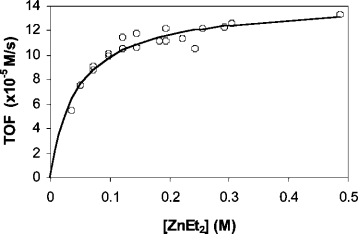
\includegraphics[scale=0.5]{TOF_vs_Et2Zn}
  \caption{TOF与Et\textsubscript{2}Zn浓度的关系。
          圆圈为实验测定值,曲线为$(\ref{eq:Ni_TOF_withConcentration})$的拟合。}
  \label{TOF_vs_Et2Zn}
\end{figure}

\section*{总结}
经过上文的讨论,我们可以有如下总结:

\textbf{1. 单纯过渡态不能决定反应速率。}TDI同样会有影响。

\textbf{2. TDTS不一定是能量最高的过渡态,TDI也不一定是能量最低的中间体。}
根据公式$(\ref{eq:TOFappro})$,TOF是由能量跨度最大的中间体和过渡态的组合决定的。
由于能量跨度要考虑\textit{"反应能"},因此具体哪个组合的能量跨度大,需要计算得出。
根据图$\ref{fig:sum_energy_span}$(A),能量最高的过渡态是$T_1$,
能量最低的中间体是$I_2$,这两个物质组合有:
$\delta{E}=T_1 - I_2 + \Delta{G}_r$。
但是该值小于$T_2$和$I_1$的$\delta{E}$。
因此在这个反应曲线中,TDI不是能量最低的中间体,TDTS也不是能量最高的过渡态。
图$\ref{fig:sum_energy_span}$(B)展示了
为什么过渡态在中间体前出现时要加上反应的$\Delta{G}_r$。
由于反应是一直向前进行的,在得到$I_2$后,反应是不能够回到$T_1$的。
因此我们在计算$T_1$和$I_2$的能量跨度时
必须将当前循环的$T_1^{i}$换为下一个循环的$T_1^{i+1}$。
下一个循环的$T_1^{i+1}$相较于当前循环的$T_1^{i}$能量加上了反应能$\Delta{G}_r$,
也就是$T_1^{i+1} = T_1^{i} + \Delta{G}_r$。
因此有$\delta{E} = T_1^{i+1} - I_2 =  T_1^{i} - I_2 + \Delta{G}_r$。
\begin{figure}[H]
  \centering
  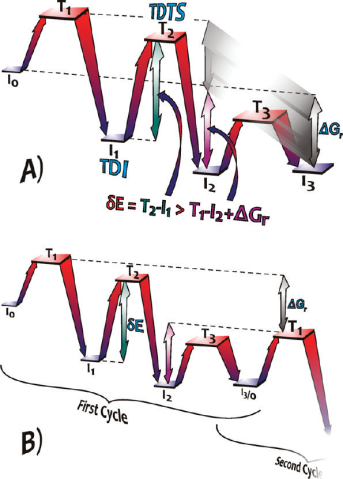
\includegraphics[scale=0.5]{sum_energy_span}
  \caption{(A)一个催化反应模型的能量曲线。(B)考虑反应能的原因示意图。}
  \label{fig:sum_energy_span}
\end{figure}

\textbf{3. 没有决定速率的步骤,只有决定速率的STATES。}
尽管人们经常认为rate-determining step(RDS)的概念有误导作用,
但是依然被一些研究人员所使用。
RDS的简单定义是整个反应中最慢的步骤。
但是根绝稳态近似理论,所有步骤的反应速率都应该是一样的。
根据IUPAC的定义:
当反应平衡常数$K$保持不变时,对整体反应速率有较大影响的速率常数$k$的步骤是RDS。
但其实我们仔细考虑一下,该定义实际上指的是rate-determining \textbf{TS}。
图$\ref{fig:no_RDS}$中哪一步是RDS?TS能量最高的第一步?活化能最高的第二步?
还是过渡态为TDTS的第四步?
答案当然是没有正确答案,因为首先“哪一步是RDS?”这个问题就不成立。; )
\begin{figure}[H]
  \centering
  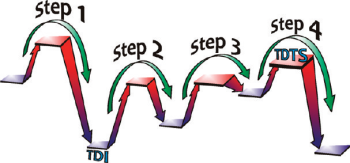
\includegraphics[scale=0.5]{no_RDS}
  \caption{“没有RDS”概念举例。}
  \label{fig:no_RDS}
\end{figure}

\section*{应用能量跨度模型的注意事项}
在得到反应的能量曲线后,能量跨度模型可以帮助我们评估反应的动力学。
但是这一模型有其应用的前提:
\circled{1}过渡态理论有效;
\circled{2}稳态近似理论可以用于该体系;
\circled{3}\footnote{原文为“fast relaxation”}中间体可以经历快速转化。

能量跨度模型的另一个局限性是:考虑到熵效应,相较于内能,
我们常常难以计算得到物质精确的自由能。
由于TDTS/TDI能量的误差对TOF的影响是指数性的,
因此目前通过计算还难以得到精确的TOF。
但是由于误差抵消的因素,TOF的相对值还是可信的。

最后一个需要注意的地方是反应有多个路线的情况下TDTS/TDI的确定。
图$\ref{competing_mechanism}$中,TDTS和TDI来自于不同的反应路线。
\begin{figure}[H]
  \centering
  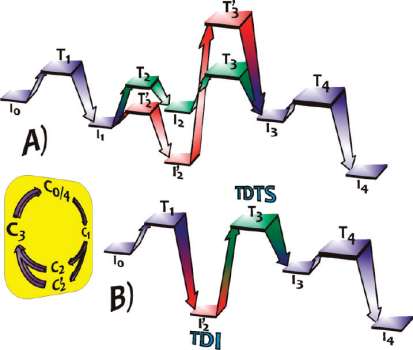
\includegraphics[scale=0.5]{competing_mechanism}
  \caption{有两个竞争路线的模型反应。}
  \label{competing_mechanism}
\end{figure}















\end{document}
